% !TEX root = DesignDoc.tex

\chapter{Electrical Design}
\label{chap:elecdesign}

This chapter details the electrical components used in the design, and includes logical connection diagrams. Provide wiring diagrams both for data flow and power. Include all components, but don't worry too much about individual pins or wires. The main point is to supply the reader with a high level description of the electrical design. Also list all of the electrical components used and provide datasheets.

\section{Parts List}

\begin{itemize}
	\item{Provide a brief summary of the parts used here}
\end{itemize}

\subsection{Part 1}

Use as many subsections as you have parts to describe the parts, their use, and provide links to datasheets. Include the datasheets with the document, rather than relying on web-links.
%\pagebreak
\section{Wiring Diagrams}

Provide two wiring diagrams. One for data, one for power.

%\subsection{Power}

%\begin{figure}[h]
%\centering
%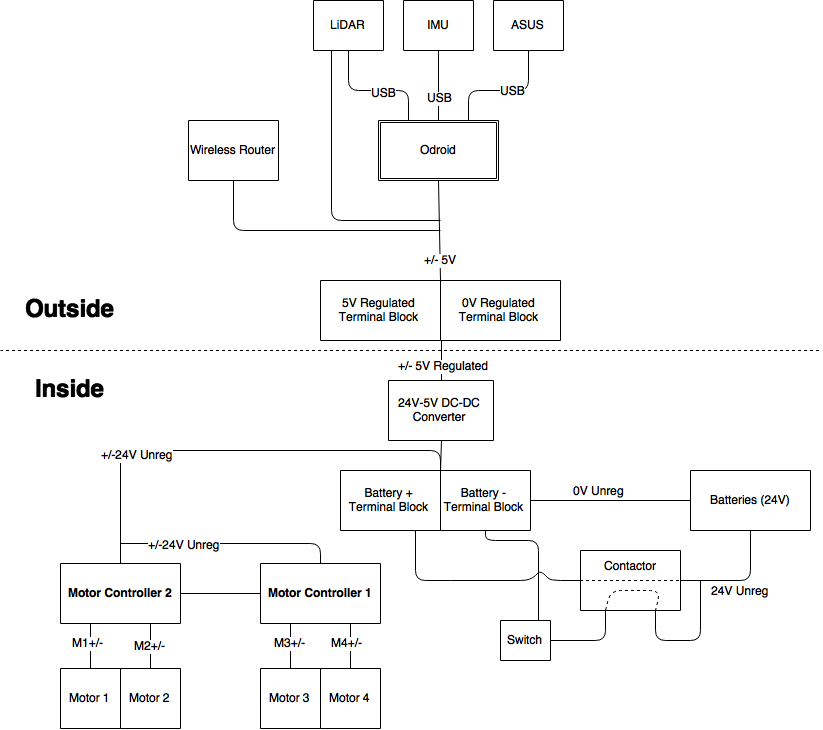
\includegraphics[width=\textwidth]{PowerDiagram.png}
%\label{fig:powerdiagram}
%\caption{Power Connections}
%\end{figure}
%\pagebreak
%\subsection{Logic}

%\begin{figure}[h]
%\centering
%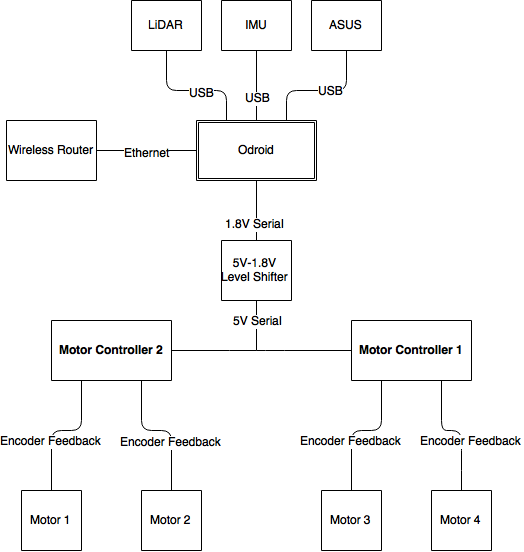
\includegraphics[width=.75\textwidth]{LogicDiagram.png}
%\label{fig:logicdiagram}
%\caption{Logical Connections}
%\end{figure}